\documentclass[tikz,border=5pt]{standalone}
\usepackage[utf8]{inputenc}
\usepackage{tikz}
\usetikzlibrary{shapes.geometric, arrows.meta, positioning, shadows.blur, calc, fit, backgrounds}

% --- Professional Colors ---
\definecolor{frameBlue}{RGB}{64, 112, 175}      % Input Framing
\definecolor{gapRed}{RGB}{214, 69, 65}          % Missing Robustness
\definecolor{lexicalOrange}{RGB}{230, 126, 34}  % Surface Cues (Process)
\definecolor{manipPurple}{RGB}{142, 68, 173}    % Manipulated Output

% --- Global Style Definitions (Prevents Compile Errors) ---
\tikzset{
    % Base Block Style
    process/.style={
        rectangle, 
        rounded corners=2mm, 
        minimum width=3.8cm,      
        minimum height=1.0cm,     
        text centered, 
        text width=3.5cm,         
        font=\sffamily\footnotesize, 
        draw=gray!40,
        thick,
        blur shadow={shadow blur steps=3}
    },
    % Specific Role Styles
    stepFrame/.style={process, fill=frameBlue!10, draw=frameBlue!80!black},
    stepGap/.style={process, fill=gapRed!10, draw=gapRed!80!black},
    stepLex/.style={process, fill=lexicalOrange!10, draw=lexicalOrange!80!black},
    stepManip/.style={process, fill=manipPurple!10, draw=manipPurple!80!black},
    % Arrow & Label Styles
    arrow/.style={-{Stealth}, thick, draw=gray!60, rounded corners},
    groupLabel/.style={font=\bfseries\sffamily\tiny, color=gray!70, anchor=north west}
}

\begin{document}

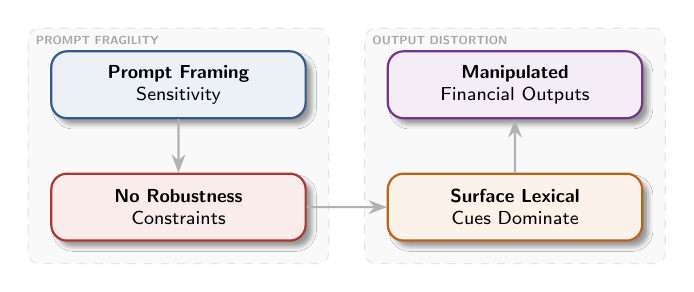
\begin{tikzpicture}[
    transform shape, 
    scale=0.85, 
    node distance=0.8cm and 1.2cm
]

    % --- LEFT COLUMN (Vulnerability) ---
    
    % 1. Framing Sensitivity (Top Left)
    \node (step1) [stepFrame] {
        \textbf{Prompt Framing} \\ 
        Sensitivity
    };

    % 2. Robustness Gap (Bottom Left)
    \node (step2) [stepGap, below=of step1] {
        \textbf{No Robustness} \\ 
        Constraints
    };

    % --- RIGHT COLUMN (Exploitation & Result) ---
    
    % 3. Lexical Cues (Bottom Right - Across from Step 2)
    \node (step3) [stepLex, right=of step2] {
        \textbf{Surface Lexical} \\ 
        Cues Dominate
    };

    % 4. Manipulated Output (Top Right - Above Step 3)
    \node (step4) [stepManip, above=of step3] {
        \textbf{Manipulated} \\ 
        Financial Outputs
    };

    % --- Arrows (The U-Shape) ---
    \draw [arrow] (step1) -- (step2);  % Down
    \draw [arrow] (step2) -- (step3);  % Across
    \draw [arrow] (step3) -- (step4);  % Up

    % --- Background Grouping ---
    \begin{scope}[on background layer]
        % Group 1: The Input Weakness
        \node [fit=(step1)(step2), fill=gray!5, draw=gray!20, rounded corners, dashed, inner sep=8pt] (groupL) {};
        \node [groupLabel] at (groupL.north west) {PROMPT FRAGILITY};
        
        % Group 2: The Failure Mechanism
        \node [fit=(step3)(step4), fill=gray!5, draw=gray!20, rounded corners, dashed, inner sep=8pt] (groupR) {};
        \node [groupLabel] at (groupR.north west) {OUTPUT DISTORTION};
    \end{scope}

\end{tikzpicture}
\end{document}